\chapter{QTor}
%\chapter{QTOR}
\label{QTOR}

%%%%%%%%%%%%%%%%%%%%%%%%%%%%%%%%%%%%%%%%%%%%%%%%%%%%%%%%%%%%%%
%\section{QTOR\index{QTOR}}
%%\noindent
%QTOR has been used in $Q^p_{weak}$ experiment for seperating elastic and inelastic events.


%%%%%%%%%%%%%%%%%%%%%%%%%%%%%%%%%%%%%%%%%%%%%%%%%%%%%%%%%%%%%
\section{Hall Probe\index{QTOR!hall probe}}
\label{Hall Probe}
%The Qtor Hall probes will be hooked up to the same Lakeshore controller that the HMS hall probes used. Nur and I took the VME IOC that was used out of the HMS hut and moved it to the doghouse. We connected IOC to the Lakeshore, and after restoring some boot information on the CPU (vmec18), the EPICS controls appear to still work.
%For now, we will use the HMS EPICS names, Q1HallP, Q2HallP and Q3HallP. The hall probes can be read from the cdaq machines with the commands:

The QTor Hall probes were hooked up to a Lakeshore controller, taken from the old HMS hut. The VME IOC inside the HMS hut was also moved to the doghouse and was connected to the Lakeshore controller. After restoring some boot information on the CPU (vmec18), the EPICS controls was used to to control the system.
The EPICS names for the Lakeshore controller outputs were Q1HallP, Q2HallP and Q3HallP. The hall probes can be read from the cdaq machines with the commands:

\noindent
\texttt{caget Q1HallP \\
caget Q2HallP \\
caget Q3HallP. \\
}

These channels were also added to the QTor GUI, that controlled the QTor power supply. 
%I will add these to the QTor GUI I am preparing.
There are EPICS commands to zero the probes:

\noindent
\texttt{caput Q1ZeroP \\
caput Q2ZeroP \\
caput Q3ZeroP. \\
}

These will send the command ``ZCAL" to the Lakeshore for the specified probe. In addition, the IOC for the Hall probe was also accessed via the portserver.


%%-----------------------------%
%
% Here is the summary for the Ethernet configuration around the doghouse.
%If you have question, please let me know.
%
%
% * Twenty-four Ethernet connections for Qweak
%
% doghouse  ----  T20 Rack    ---- PANEL A ---- Fiber Optic Slot(FOS)
%  cable \#         Patch Panel      HC01Z04      Netgear or hallc-cat2950
%   1              1                1            FOS 6
%   2              2                2            FOS 16
%   3              3                3            FOS 10
%   4              4                4            FOS 17
%   5              5                5            FOS 18
%   6              6                6            FOS 19
%   7              7                7            FOS 20
%   8              8                8            FOS  5
%   9-15           9-15             9-15         1-7 (Netgear switch)
%   16-24          16-24            16-24        available ports on
%                                                hallc-cat2950 (cisco)
%
%
%  * Detailed use of T20 Rack Patch Panel \#
%
%   FOS
%   1  -------- Reserved   (Boot Power Strip for ROC9)
%   2  -------- Reserved   (Boot Power Strip for ROC10)
%   3  -------- hcreboot13 (Boot Power Strip for others)
%   4  -------- hctsv11    (portserver)
%   5  -------- IOC for Hall Probe        (hctsv11 2002)
%   6  -------- qwvme9     (CPU of ROC9)  (hctsv11 2008)
%   7  -------- qwvme10    (CPU of ROC10) (hctsv11 2007)
%   8  -------- qwvme11    (CPU of ROC11) (hctsv11 2006)
%
%   Netgear
%   9  -------- qwvme9mon  (ROC9 crate Power Monitor)
%   10 -------- qwvme10mon (ROC10 crate Power Monitor)
%   11-15       Reserved   (connected to the doghouse)
%
%   Cisco
%   16 -------- qwscannerctrl (scanner controller unit)
%   17-22       Reserved   (not connected)
%   23 -------- a Netgear 4port switch (doghouse, temp?)
%   24 -------- region 3 rotator controller
%
%   In addition, I checked the IOC for the Hall probe via the portserver as
%
%   [VxWorks Boot]: p
%   boot device          : ei
%   processor number     : 0
%   host name            : cdaqs3
%   file name            : ~/KERNELS/vx162
%   inet on ethernet (e) : 129.57.168.118:fffffc00
%   host inet (h)        : 129.57.168.16
%   user (u)             : cvxwrks
%   flags (f)            : 0x20
%   target name (tn)     : vmec18
%   startup script (s)   : ~/SCRIPTS/vmec18.boot
%   
%%-----------------------------%
%

\begin{figure}[h]
	\begin{center}
		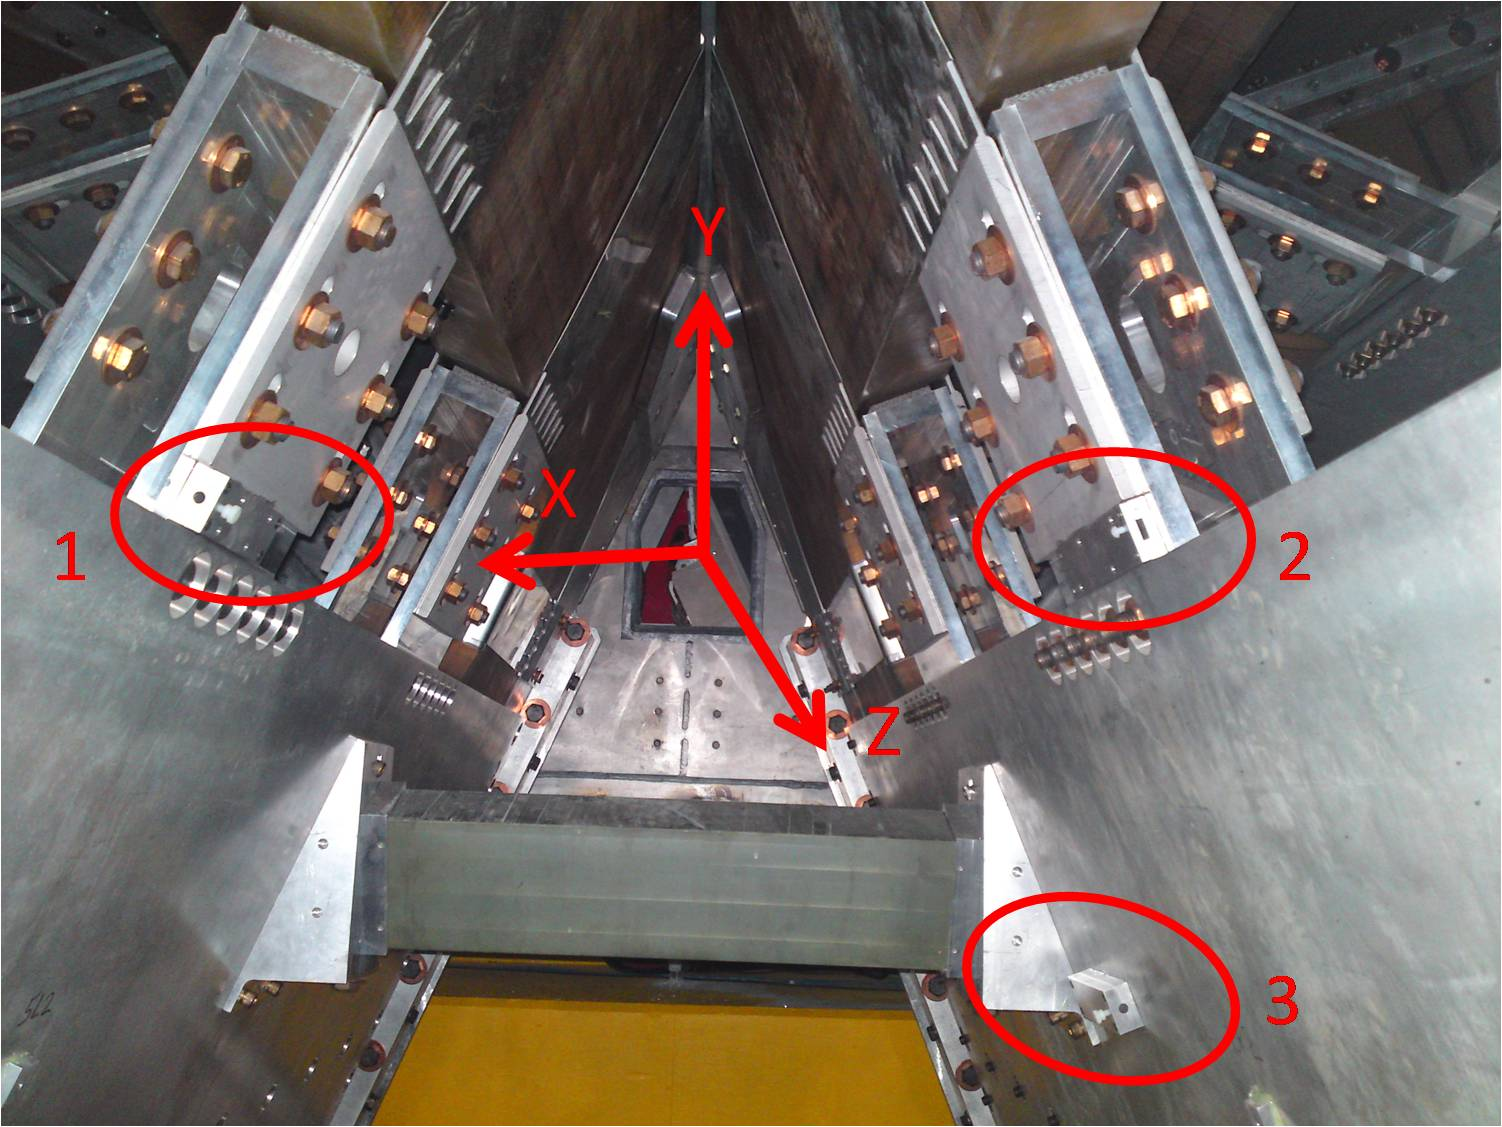
\includegraphics[width=14.5cm]{figures/qtor_hallprobe_mount}
		\label{fig:qtor_hallprobe_mount}
		\caption
%		[QTor hall probe locations.]
		{QTor hall probe mounts and their locations inside the QTor are shown here.}
	\end{center}
\end{figure}


%%%%%%%%%%%%%%%%%%%%%%%%%%%%%%%%%%%%%%%%%%%%%%%%%%%%%%%%%%%%%
\section{QTor Corrector Magnet\index{QTor!Corrector magnet}}
\noindent
The idea of this analysis is to estimate beam steering due to QTOR fringe field assuming a field of
4500 Gauss-cm along the beam axis using OPTIM.

Recently we discovered QTOR steers the forward beam. We tried to examine whether this steering is
due to expected QTOR fringe field along the beam axis, or it indicates misalignment or motion of any QTOR coils. The steering implies a field integral of 4500 Gauss-cm. See more details in [1]. In this analysis we tried to predict the effect of QTOR fringe field (4500 Gauss-cm) along the beam axis Using OPTIM simulation.


\subsection{TOSCA\index{TOSCA}}
\label{TOSCA}


\begin{figure}[h]
	\begin{center}
		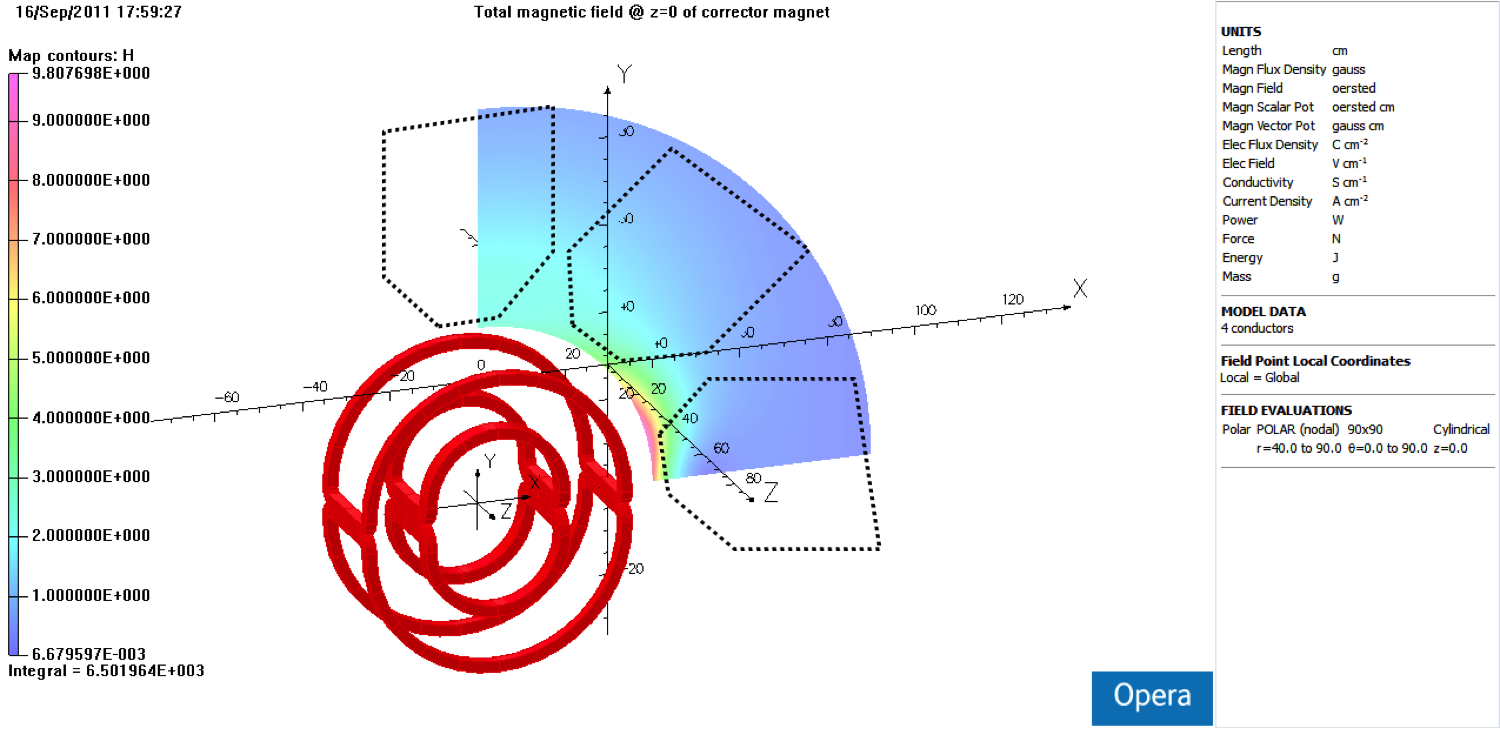
\includegraphics[width=15.0cm]{figures/qtor_corrector_field_z0}
	\end{center}
		\caption
%		[The QTor corrector magnet design and magnetic field for an octant at Z=0.]
		{The QTor corrector magnet design and magnetic field for an octant at Z=0. The primary collimator openings are also shown in the figure. The magnetic fields along the collimator openings are simulated. }
		\label{fig:qtor_corrector_field_z0}
\end{figure}

\begin{figure}[h]
	\begin{center}
		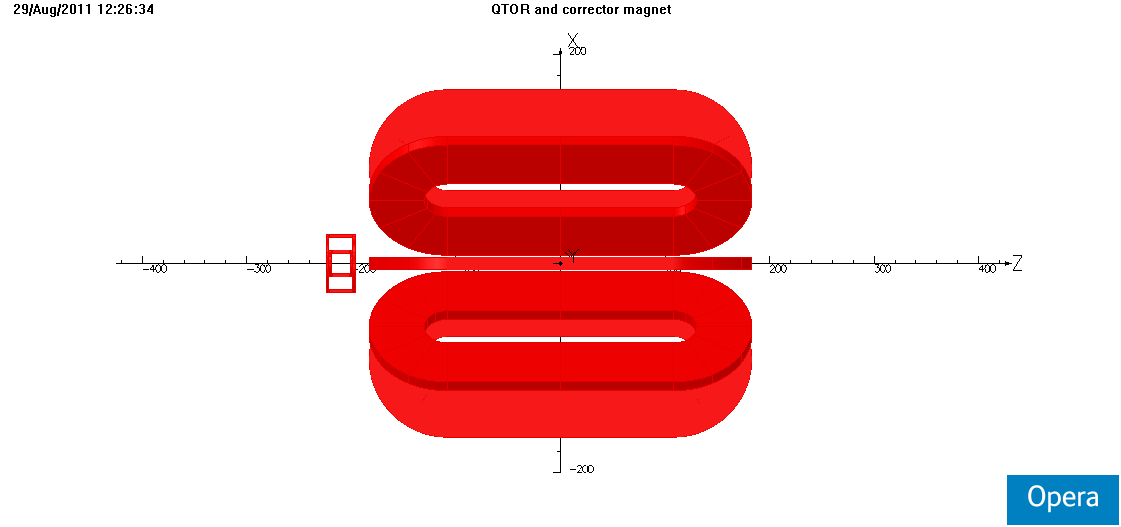
\includegraphics[width=15.0cm]{figures/qtor_corrector1}
	\end{center}
		\caption
%		[The QTor with its corrector magnet from side view.]
		{The QTor with its corrector magnet from side view.}
		\label{fig:qtor_corrector1}
\end{figure}


\begin{figure}[h]
	\begin{center}
		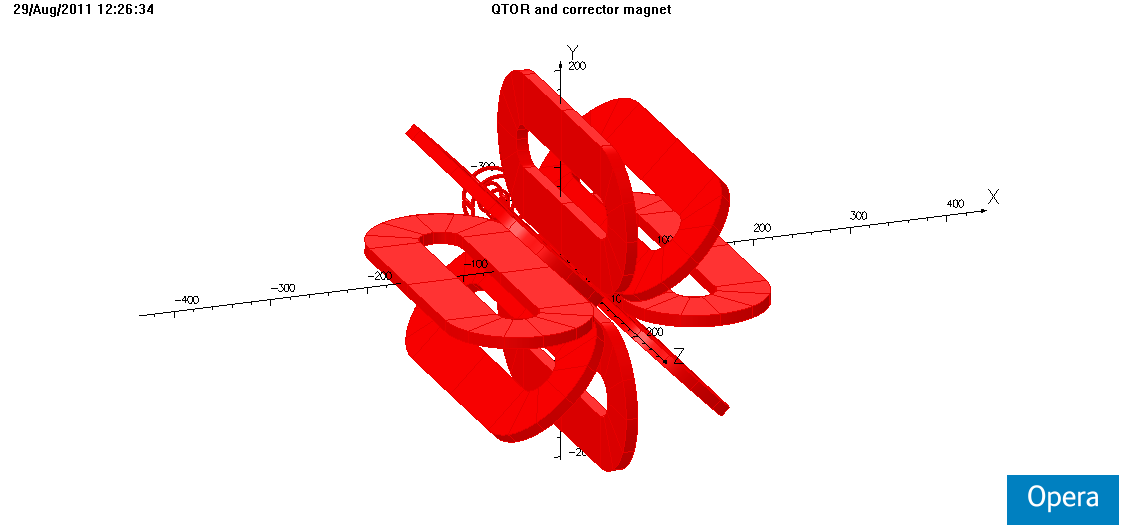
\includegraphics[width=15.0cm]{figures/qtor_corrector3}
	\end{center}
		\caption
%		[The QTor with its corrector magnet.]
		{A three-dimensional view of the QTor with its corrector magnet.}
		\label{fig:qtor_corrector3}
\end{figure}


%We have already seen QTOR steers the forward beam due to fringe field [1, 2]. We have predicted the
%effect of QTOR fringe field (4250 Gauss-cm) along the beam axis using OPTIM simulation [2] and supported Rob�s pencil model. In this analysis we want to approach further and want to investigate the different effects of this fringe field on low energy electrons.
%
%* QTOR and dump viewer in the OPTIM model has been added for this analysis. See details in [2].
%
%* No microscopic model of the QTOR field symmetry breaking was used. We treated the QTOR region as a 4m long dipole with Rob's suggested field integral, confirming his estimate.
%
%* Earth�s magnetic field has not been considered in the model.
%
%
%Low energy electron scattering due to 4250 G-cm field at QTOR magnet. The points are fitted with
%polynomial 2. The horizontal axis is shows the different beamline element. The Q-weak target is at zero and beam is coming from left. Different energies are shown in different colors (Colors are chosen according to energy. Convention is Violet � 1162 [nominal], Indigo � 1000, Blue � 750, Green � 500, Orange � 250 and Red � 100 MeV). As expected low energy electrons are deflected much more than high energy electrons. 
%
%Motivation: We have already seen QTOR steers the forward beam due to fringe field [1, 2]. We have predicted the effect of QTOR fringe field (4250 Gauss-cm) along the beam axis using OPTIM simulation [2,3]. In this analysis we want to add a corrector magnet in front of QTOR and investigate the effects of this magnet on fringe field on electrons.
%
%Figure 1: Beam trajectory after applying ZERO filed in the corrector magnet in front of QTOR. 
%
%Figure 2: Beam trajectory after applying a filed of 4000 G-cm in the corrector magnet in front of QTOR. Its mainly focusing the trajectories at the dump viewer. 
%
%Figure 3: Beam trajectory after applying a filed of 4000 G-cm in the corrector magnet in front of QTOR to focus at the dump viewer. Same as Figure 2, just a zoomed in version for better visualization.
%
%Figure 4: Beam trajectory after applying a filed of 4288 G-cm in the corrector magnet in front of QTOR. Its mainly focusing the trajectories at the dump window. 
%
%Figure 5: Beam trajectory after applying a filed of 4288 G-cm in the corrector magnet in front of QTOR to focus at the dump window. Same as Figure 4, just a zoomed in version for better visualization.
%
%We have investigated the effects of a magnet in front of QTOR on different energy electrons [4]. In
%this analysis we want to vary the  magnetic field of corrector magnet in front of QTOR and investigate the
%effects of this field variation on electrons.
%
%Figure 1: Beam trajectory due to different fields in the corrector magnet for a single energy electrons. Then the plot is animated over different beam energies. The beam energy is written on the headings of the plots and different magnetic fields are shown in different colors and symbols are shown in the legend section (right hand side) of the plots. 
%
%At the end we may not approach for a magnet in front of QTOR due to its far field effect. Later we may search for a different place (most likely downstream, as we don't have enough space upstream of QTOR) rather than just before QTOR.
%
%
%
%Motivation: We found QTOR steers the forward beam most probably due to misalignment of QTOR coils [1]. We have already investigated the effects of a magnet in front of QTOR for primary beam as well as for different energy Moller electrons [2, 3, 4 and 5]. Here we tried to design a magnet we discussed in [4] and [5].
%
%Figure 1: 3D view of QTOR corrector magnet. The current directions for the coils are shown by the arrows. 
%
%Figure 2: QTOR corrector magnet along YZ plane. Length along Z-direction (available space for magnet is 25.4 cm) is shown in this figure.
%
%Figure 3: QTOR corrector magnet along XY plane. Magnetic field perpendicular to Z- plane is also shown in a polar patch of radii 40 � 90 cm.
%
%Figure 4: QTOR corrector magnet field integral along a line in Z- direction (from -50 to +50 cm) at X = 40 cm and Y = 0 cm.
%
%Figure 5: QTOR corrector magnet field integral along a line in Z- direction (from -50 to +50 cm) at X = 0 cm and Y = 40 cm.
%
%Figure 6: QTOR corrector magnet field integral along a line in Z- direction (from -50 to +50 cm) at X = 28.3 cm and Y = 28.3 cm (diagonal).
%
%Figure 7: QTOR corrector magnet field integral along a line in Z- axis (from -50 to +50 cm).
%
%Figure 8: Possible QTOR corrector magnet location. The arrow represents beam direction.
%
%Motivation: We discussed our corrector magnet design in [1]. Here we tried to calculate the power dissipation, voltage drop and temperature rise and other important parameters of the coils. 
%
%Motivation: We showed our corrector magnet design in [1]. Here we tried to get an estimate of corrector magnet sensitivity to position or angle using TOSCA. 
%
%
%Motivation: Corrector magnet design has been shown in [1]. We tried to see the profile of magnetic field along the line of collimator opening using TOSCA. ~\ref{OPTIM}
%
%%\begin{figure}[!h]
%%	\begin{center}
%%%		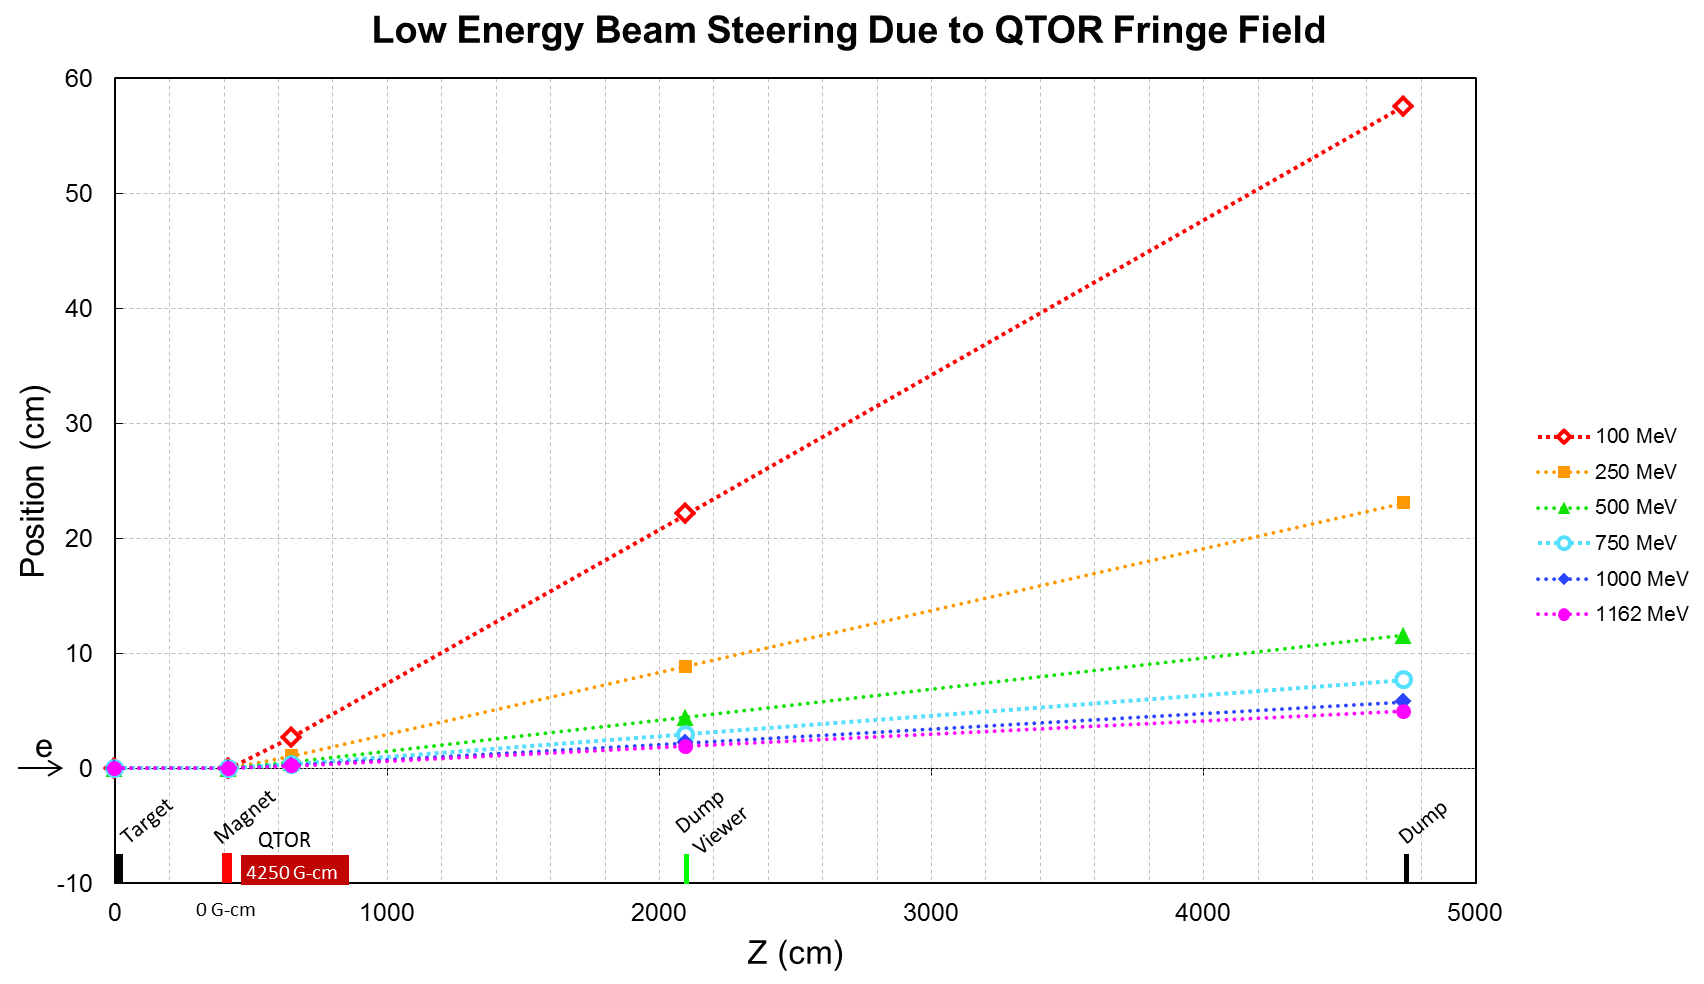
\includegraphics[trim=0.1cm 0.1cm 0.1cm 0.1cm, clip=true,width=14.5cm]{figures/qtor_allenergy_0Gcm}
%%		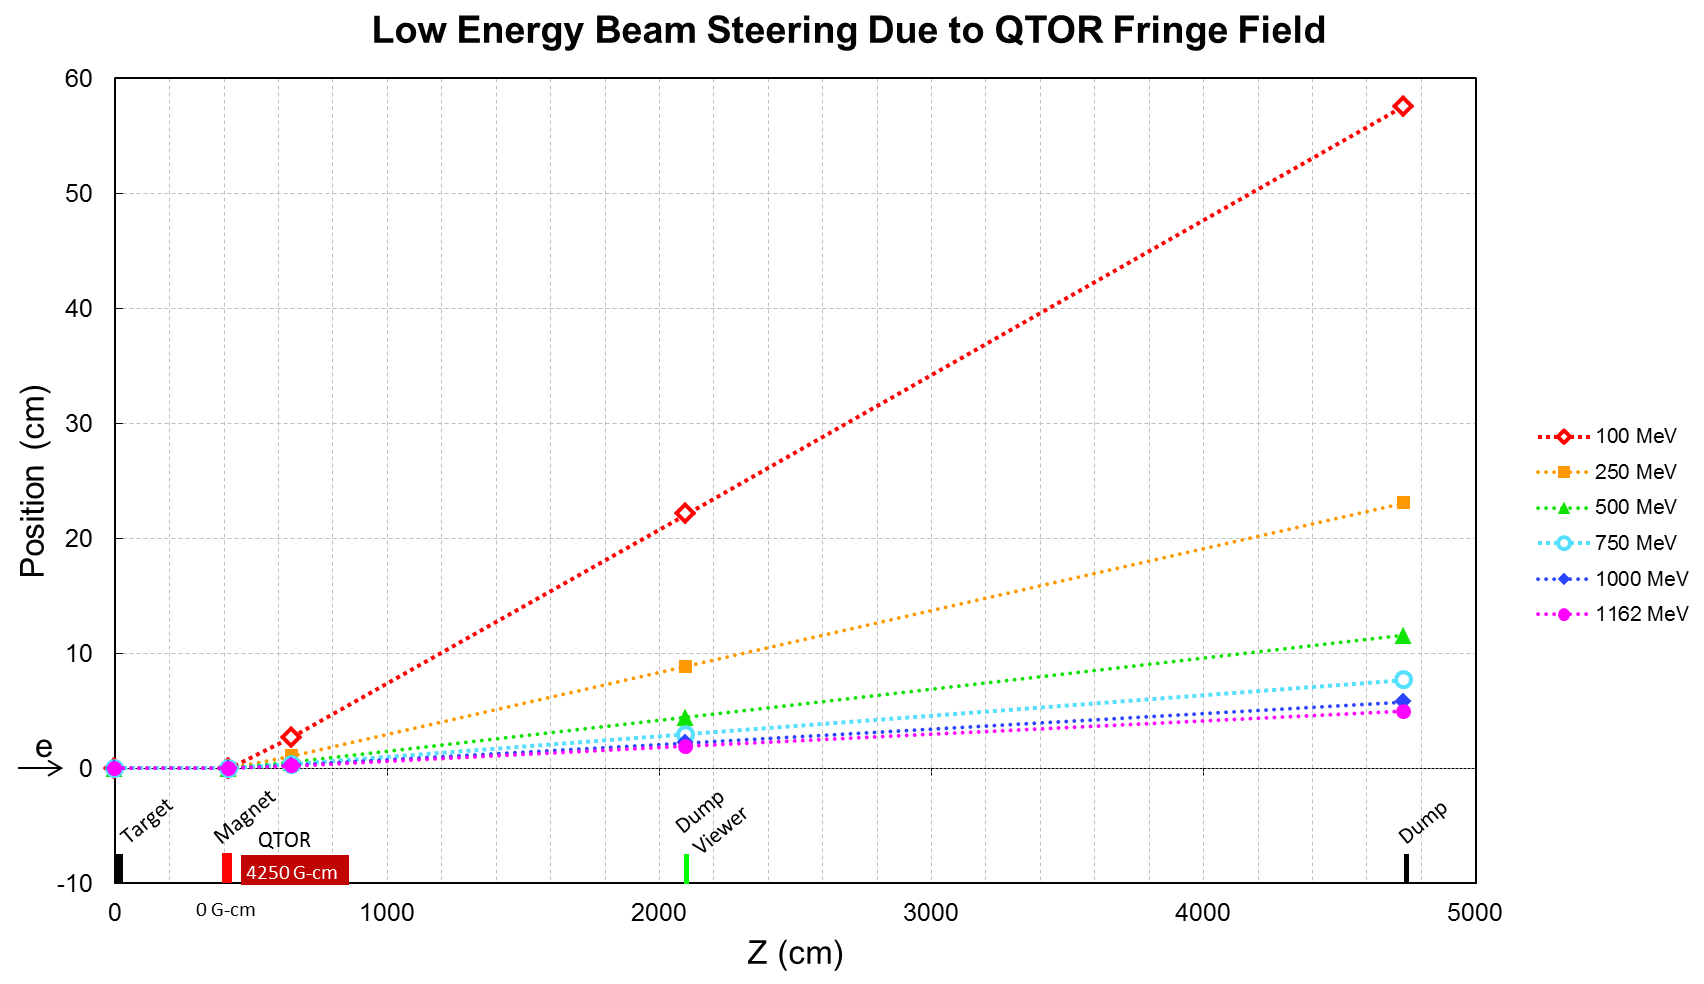
\includegraphics[width=15.0cm]{figures/qtor_allenergy_0Gcm}
%%	\end{center}
%%		\caption
%%		[QTor allenergy 0Gcm.]
%%		{QTor allenergy 0Gcm.}
%%		\label{fig:qtor_allenergy_0Gcm}
%%\end{figure}

\begin{figure}[!h]
	\begin{center}
		\includegraphics[width=15.0cm]{figures/qtor_allenergy_4000Gcm_sacle_viewer}
	\end{center}
		\caption
%		[QTor all energy 4000Gcm at the dump viewer.]
		{The trajectory of scattered electrons 4000Gcm QTor fringe field at the dump viewer.}
		\label{fig:qtor_allenergy_4000Gcm_sacle_viewer}
\end{figure}


\begin{figure}[!h]
	\begin{center}
		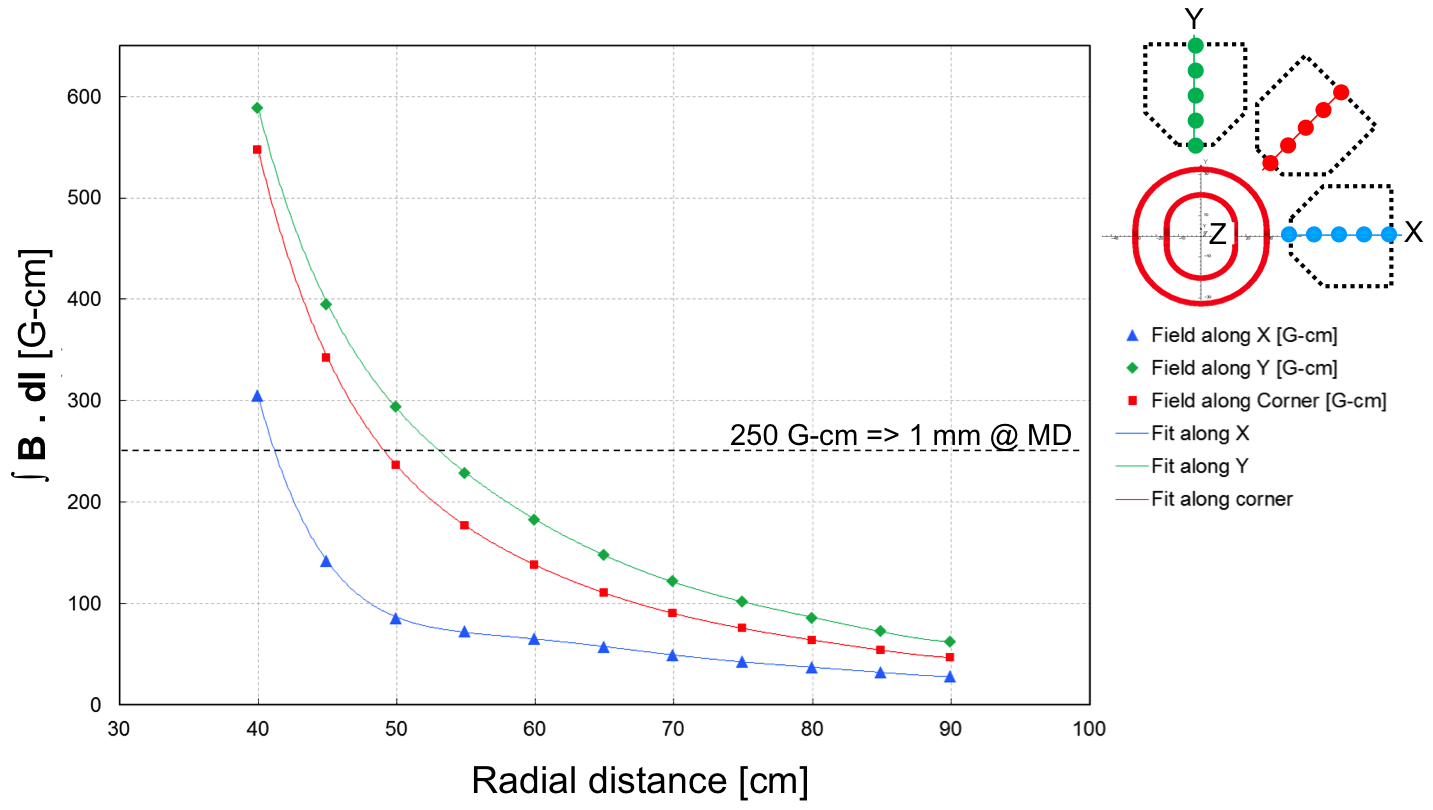
\includegraphics[width=15.0cm]{figures/qtor_corrector_field_integral_variation}
	\end{center}
		\caption
%		[QTOR qtor corrector field integral variation.]
		{The QTor corrector field integral variation along the radial direction.}
		\label{fig:qtor_corrector_field_integral_variation}
\end{figure}

\begin{figure}[!h]
	\begin{center}
		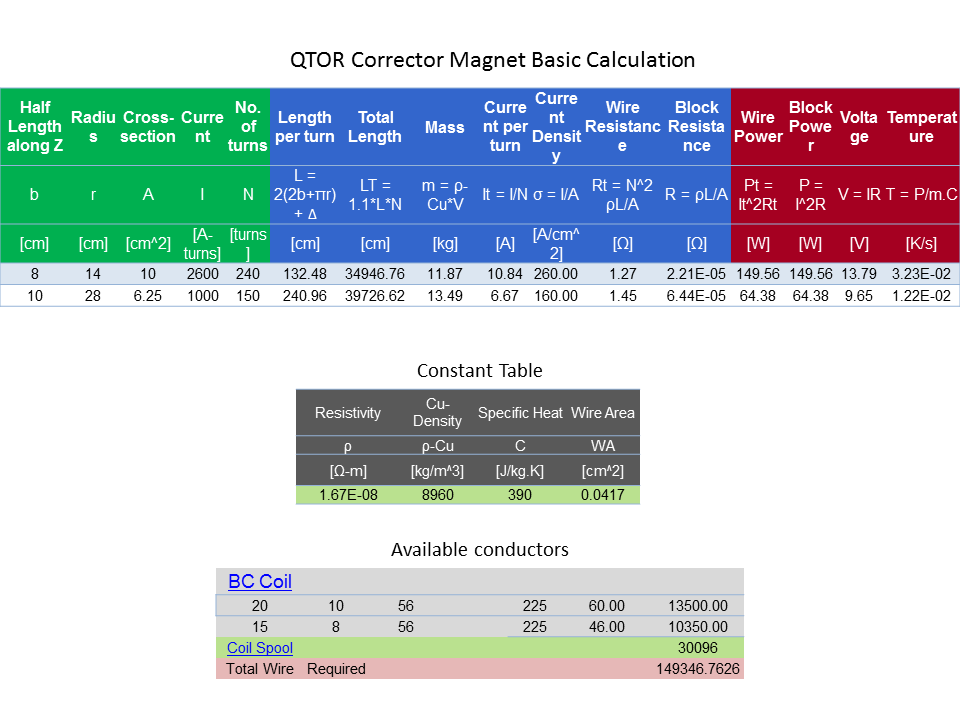
\includegraphics[width=15.0cm]{figures/qtorCorrectorMagnet_powerCalculation}
	\end{center}
		\caption
%		[The QTor corrector magnet power dissipation calculation.]
		{The QTor corrector magnet power dissipation calculation.}
		\label{fig:qtorCorrectorMagnet_powerCalculation}
\end{figure}

\begin{figure}[!h]
	\begin{center}
		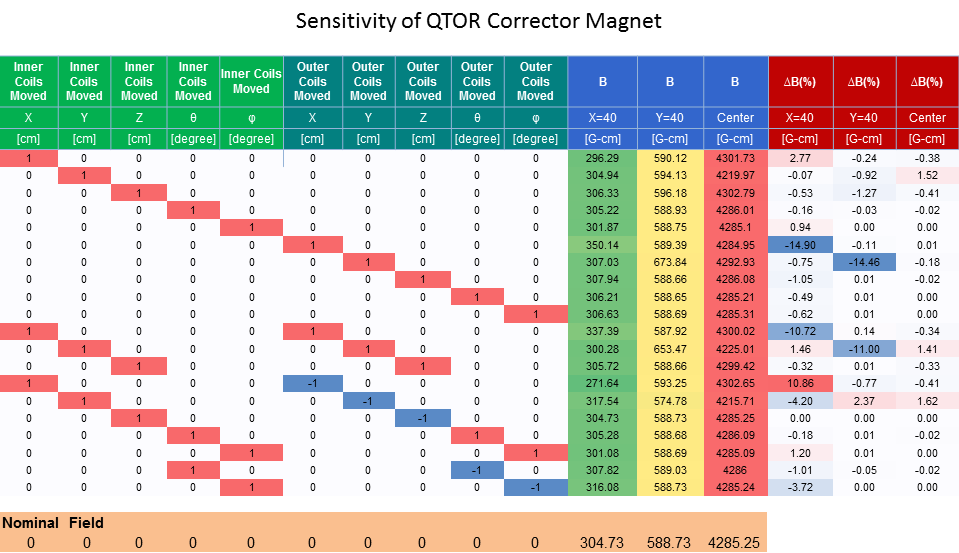
\includegraphics[width=15.0cm]{figures/qtorCorrectorMagnet_sensitivity}
	\end{center}
		\caption
%		[The QTor corrector magnet sensitivities to the position and angle change.]
		{The QTor corrector magnet sensitivities to the position and angle change.}
		\label{fig:qtorCorrectorMagnet_sensitivity}
\end{figure}



\begin{figure}[!h]
	\begin{center}
		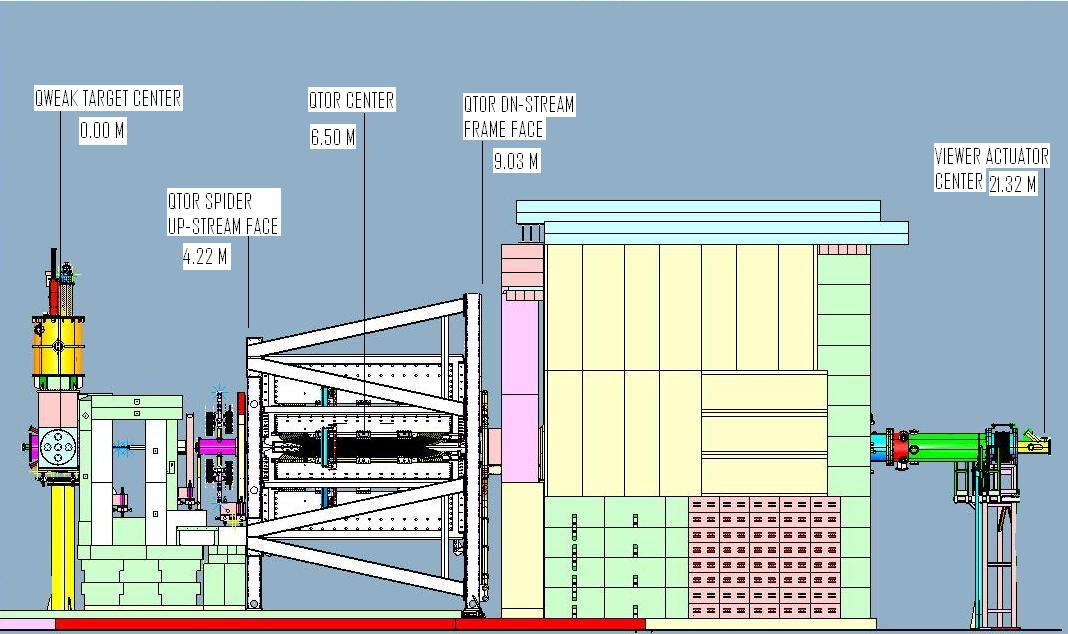
\includegraphics[width=15.0cm]{figures/qtor_cad}
	\end{center}
		\caption
%		[A Computer-aided design (CAD) of the QTor and nearby region.]
		{A Computer-aided design (CAD) of the QTor and nearby region.}
		\label{fig:qtor_cad}
\end{figure}
